% Preamble
% ---
\documentclass{article}

% Packages

% \usepackage{graphicx}
% \usepackage{subfig}

\usepackage{multicol}
\usepackage{float}

\usepackage{tikz}
\usepackage{pgfplots}
\usepgfplotslibrary{external}
% \usetikzlibrary{shapes.geometric, arrows}
% 
\usepackage[english]{babel}
\usepackage{hyperref} % 1 -> Figure 1
\usepackage{caption}

% code block
\usepackage{xcolor}
\usepackage{listings}

\definecolor{mGreen}{rgb}{0,0.6,0}
\definecolor{mGray}{rgb}{0.5,0.5,0.5}
\definecolor{mPurple}{rgb}{0.58,0,0.82}
\definecolor{backgroundColour}{rgb}{0.95,0.95,0.92}

\lstdefinestyle{CStyle}{
    backgroundcolor=\color{backgroundColour},   
    commentstyle=\color{mGreen},
    keywordstyle=\color{magenta},
    numberstyle=\tiny\color{mGray},
    stringstyle=\color{mPurple},
    basicstyle=\footnotesize,
    breakatwhitespace=false,         
    breaklines=true,                 
    captionpos=b,                    
    keepspaces=true,                 
    numbers=left,                    
    numbersep=2pt,                  
    showspaces=false,                
    showstringspaces=false,
    showtabs=false,                  
    tabsize=2,
    language=C
}

\pgfplotscreateplotcyclelist{mylist}{%
red,every mark/.append style={fill=red!80!black},mark=*,mark size=3pt\\%
brown!60!black,every mark/.append style={fill=brown!80!black},mark=*, mark size=3pt\\%
black,every mark/.append style={fill=black!80!black},mark=*, mark size = 3pt\\%
}


\usepackage{geometry}
\geometry{margin=1.2cm}

% ---

% \graphicspath{ {assets/} }

% \setlength{\columnsep}{1.3cm}

% \setlength{\columnsep}{0.8cm}
\begin{document}
\begin{multicols}{2}

\section{Introduction}

This report will the explore the optimizations applied to the implementation of
the d2q9-bgk lattice boltzmann scheme. It will initally look at the serial
omtimizations and how they affected the performance of the alogirthm It will
then look at the parallel implementation and how this affect the performance
with different number of cores and problem sizes.

\section{Serial Optimisation}

\subsection{Compiler options}

Many modern compilers provide various options to optimize the given code. 

\autoref{tab:compilerflags} shows the run time of the serial optimized code
(without vectorization) with different compiler flags. This shows that by
simply using the \verb|-Ofast| flag there can be a 4x decrease in run time. The
\verb|-mtune=native| option can further imporve the performance by telling the
compiler to optimize the code for the specific local machine and its
instruction set. The compiler flag \verb|-no-prec-sqrt| was also used, which
reduces the required precision of the square root funciton which is used in the
critical section of the algorithm.

\begin{center}
  \begin{tabular}{ |p{5cm}||p{1.5cm}| }
 \hline
 \multicolumn{2}{|c|}{Results} \\
 \hline
 Compiler flag & Run time \\
 \hline
 -O0                  & 111.7   \\
 -O1                  & 34.5   \\
 -O2                  & 34.2   \\ 
 -O3                  & 31.9   \\ 
 -Ofast               & 26.8   \\ 
 -Ofast -mtune=native & 26.5   \\
 \hline
\end{tabular}
\captionof{table}{Serial run time with different compiler flags}
\label{tab:compilerflags}
\end{center}

\subsection{Reduce Memory Accesses}

In the original implementation of the algorithm for each timestep the
\verb|cells| array was looped over the 4 times, in \verb|propagate|,
\verb|rebound|, \verb|collision| and \verb|av_velocity|. This resulted in
repeated stores and loads of the same sections of memory. To prevent this the
first 3 separate functions (those in the \verb|timestep| function) were fuzed
into a single loop. This meant the same sections of memory were used closer
together making it is more likely for them to still be in cache. The function
\verb|av_velocity| was then repeating calculations that already took place in
collision and requiring an additional loop over cells. The result was therefore
calculated in the single parse over the cells and returned from the timestep
function. Similarly in propagate and collisions the values were switched
between \verb|tmp_cells| and \verb|cells| multiple times. In the new
implementation the \verb|tmp_cells| array was used as the "answer" space and
stored only the next timesteps cell values. This then only required a single
write to \verb|tmp_cells| each timestep. At the end of the timestep the
\verb|tmp_cells| and \verb|cells| array's pointers were then swapped which set
the \verb|cells| array to the correct value without having to write directly to
the array.

\subsection{Vecotrisation}

Having improved the implementation of the serial code, there is now a clear
critical section of the code, inside the single pass of the cell. This is where
the majority of the computation takes places and thus is where most of the time
of the program is used. Since this section performs multiple mathematical
computation on the input array, there is an additional approach to optimization
other than parallelizing it. This is approach makes use of SIMD,
(single-instruction multiple data). This is where compilers are able to use
vector registers and instructions to make multiple computations on a chuck of
data (a vector) with a single instruction. This has the potential for large
performance gains as fewer instructions are required for the cells array.

\begin{lstlisting}[style=CStyle, label={lst:cellsdataalign}, caption={Example of memory allignment for a cells array.},]
  // Allocate aligned data
  cells_ptr->speed0 = _mm_malloc(params->nx * params->ny * sizeof(float), 64);
  // When using the array allow the compiler to assume alignment
  __assume_aligned(cells->speed0, 64);
\end{lstlisting}

% TODO should I reference the proluge step
In many cases the compiler is able to automatically vectorize code blocks.
However if the data is not aligned then the compiler will have to complete a prior
step, called the "prologue" step to process this unaligned data, or
alternatively use unaligned instructions (which are less efficient). The
compiler is also not able to assume that an array of floats, such as the arrays
of speeds in the new \verb|t_speed| struct are aligned. Therefore it will have
to complete this prior step regardless. To prevent this the arrays can be
aligned when they are created using the \verb|__mm_malloc| function, as shown in \autoref{lst:cellsdataalign}. This
ensure the created array is aligned on the request boundry, in this case 64
bytes was used to match the size of the cache line in an \emph{intel xeon
e5-2680}. Compiler directives can then be use to tell the compiler the arrays
are aligned. This allows the compiler to skip the "proluge" step and use the
aligned instructions.


% TODO Reference wiki or find anther definition of write own definition
Another useful hint to assist the compiler in its optimizations is to use the
\verb|restrict| keyword. This tells the compiler "that for the lifetime of the
pointer, only the pointer itself or a value directly derived from it (such as
pointer + 1) will be used to access the object to which it points". In
practical terms this reduces the number of times the pointer value has to be
fetched from memory as the cached value can be used repeatedly. In a memory
bound problem this can therefore be an important step in reducing the memory
bandwidth used.

\begin{lstlisting}[style=CStyle, label={lst:assumecellssize}, caption={Additional compiler hints},]
  __assume(params.nx%128==0);
  __assume(params.ny%128==0);
\end{lstlisting}

The intel compiler also allows for other hints to be provided. In this
implementation hints were porivded to inform the compiler about the size of the
cells array (and therefore the size of the loops). As show in the example in
\autoref{lst:assumecellssize}, the \verb|__assume| directive was used, to tell
compiler that the size of the cells array was divisible by a given power of 2.
In the implementation all powers of 2, up to a maximum of 128 were provided (as
this was the maximum input size). This should further assist the compiler in
its optimizations, especially when vectorizing the inner loop.

The final step to ensuring the code was vectorized was to add the compiler
directive \verb|#pragma omp simd| to the inner for loop. This explicitly tells
the compiler that this section of the code should be vectorized. 

% TODO get some results for this
Having completed the above steps only a minor improvement in performance were
observed, as seen in Figure xx, despite the inner loop being successfully
vectorized. From the roofline graph in Figure xx, it is clear that the code was
memory bandwidth bound. In this case the problem arose from the data layout used for the cells.

In the original implementation the speeds for each cell were stored in a
structure (\verb|t_speed|) and the whole grid of cells was an array of these
structures. This implementation does not lend it self to vetorization as it
can result in unnecessary fetches from memory. This is because when a single
speed value is fetch an entire cache line (64 bits) will be used to fetch the
structure. This results in a waste of memory bandwidth as the rest of the
cache line is not used (only the single float value for that speed is actually
required). Therefore switching the implementation to use a structure of arrays
(where each speed is a separate array) allowed the code to be vectorized more
efficiently as each fetch for a speed only fetched a single float and therefore
reduced the memory bandwidth required. 

\begin{tikzpicture}
\begin{axis}[
  xmode = log,
  ymode = log,
  axis lines = left,
  xlabel = Operational Intensity (FLOPS/byte),
  ylabel = Double precision GFLOPS/s (Scalar),
  ymin = 1e-2,
  xmin = 0.0029,
  ymax = 1000,
  xmax = 1,
  scaled ticks=true,
  legend pos=south east,
  cycle list name=mylist
]

% Original implementation 
\addplot coordinates {
  (0.457, 4.911)
} node[below right, ] (TextNode) {$(0.46, 4.91)$};
\addlegendentry{Serial (Original Implementation)}

% Serial (No vectorizing)
\addplot coordinates {
  (0.341, 2.492)
} node[below right, ] (TextNode) {$(0.34, 2.49)$};
\addlegendentry{Serial (No vectorization)}

% Serial (No vectorizing)
\addplot coordinates {
  (0.383, 13.206)
} node[below right, ] (TextNode) {$(0.38, 13.2)$};
\addlegendentry{Serial (With vectorization)}

%DRAM
\addplot[color=blue] coordinates {
  (0.0029, 0.21)
  (0.77, 57.29)
  (100, 57.29)
} node[near start, above, sloped] (TextNode) {DRAM, 75GB/s};

%L1
\addplot[color=blue] coordinates {
  (0.0029, 25.07)
  (0.0065, 57.29)
  (100, 57.29)
} node[near start, above, sloped] (TextNode) {L1, 8830/s};

\end{axis}
\end{tikzpicture}

\begin{tikzpicture}
\begin{axis}[
  xmode = log,
  ymode = log,
  axis lines = left,
  xlabel = Operational Intensity (FLOPS/byte),
  ylabel = Double precision GFLOPS/s (Scalar),
  ymin = 0.5e-6,
  xmin = 0.5e-6,
  ymax = 10000,
  xmax = 100,
  scaled ticks=true,
  legend pos=south east,
  cycle list name=mylist
]

% Critical section
\addplot coordinates {
  (0.382, 119)
} node[below right, ] (TextNode) {$(0.382, 119)$};
\addlegendentry{28 cores parallel}

%DRAM
\addplot[color=blue] coordinates {
  (4.25e-7, 3.18e-5)
  (22.2, 1656)
  (100, 1656)
} node[midway, above, sloped] (TextNode) {DRAM, 75GB/s};
%
%L1
\addplot[color=blue] coordinates {
  (4.25e-7, 0.0032)
  (0.19, 1656)
  (100, 1656)
} node[midway, above, sloped] (TextNode) {L1, 8830GB/s};

\end{axis}
\end{tikzpicture}

\section{Parallel (OpenMP)}

Having optimized the inner loop in the above section the next optimization that
can be used is parallelizing. In this implementation the outer loop was
parallelized while the inner loop maintained the other optimizations. This was
achieved using OpenMP. This is library provided a collection of compiler
directives which can be used to write parallel shared memory programs.

The first step to making the outer loop run in parallel is to use the
\verb|parallel| and \verb|for| constructs and turn on OpenMP for the compiler with the
\verb|-fopenmp| flag. The \verb|parallel| directive tells the compiler to run
the preceding for loop in parallel and \verb|for| tells it to distribute the
work evenly across the threads.

It is then important to handle the memory sharing that takes place in the loop.
Since the \verb|av_velocity| is also calucated in this loop each loop is
required to calculate the total number of cells without obstacles and the sum
of the magnitude of the velocity for these cells. This requies a shared sum
across all the threads. Do efficiently calculate these shared sums a
\verb|reduction| is required. The \verb|reduction| directive tells the compiler
that the given varible is going to accumulated over the duration of the loop.
This allows each thread to calulate is own sum without having to syncronise the
global shared value on every write. Once the fork is complete and the threads
syncronise then all the sums can be combined to determine the final value of
the accumulated varibles. 

Another cocnsideration when writing a parallel program is the number of cores
to use. In a bluecrystal node there are 2 sockets, which house 2 \emph{intel
xeon e5-2680} CPUs. Each of these CPUs have 14 cores, giving a total of 28
cores per node. \autoref{tab:parallelresults} and \autoref{fig:parallelresults}
shows the run times of the parallel code on different numbers of cores. In the
larger problems (1024x1024) it is clear that as the number of cores increase
the run time decreases. This is as a result of the work in the critical section
being shared over a larger pool of cores and thus the forked time is decreased.
However in the smaller probelms there is a reduction in run time around 14
cores. This is observed as once the core count is above 14, memory sharing
between the sockets is required. This is where a shared section of memory is in
the cache of one the other socket so the request has to be routed through the
other socket. This takes appoximately 2x as long as fetching from the socket's
local cache. For this reason when running the alogirthm on the smallest cells
% TODO Make this a real thing
size (128x128) only 14 cores were used.

In general this non-uniform memory access, NUMA, can be mitigated by pinning 
the threads to a specific core. Setting \verb|OMP_PROC_BIND| to \verb|close|
tells OpenMP to bind the threads to specific cores and also as the threads are
assigned, ensure they are assigned to the threads closest to the master (main)
thread. Also assigning \verb|OMP_PLACES| to \verb|cores| ensures that each
thread is used as a single place (and no thread sharing occurs such as
hyper-threading). Although the threads are now pinned to individual cores this
does not mean that the NUMA problem is reduced. This is because during the
memory assignment, in the \verb|initialise| function, the initial values for the
cells array are assigned serially (on a single thread). This means all the
values will in exist the same cache, linked to this single NUMA region. This
can be prevented by ensuring the initialisation of the values is parallelised
in the same way as the it is accessed in the critical region. In this case this
means also using the \verb|#pragma omp parallel for| when assigning the initial
values to the cells array. This will ensure the data is allocated in the same
NUMA region to which it is going to be required in the critical loop.

\begin{lstlisting}[style=CStyle, label={lst:ompparallelloop}, caption={TODO},]
#pragma omp parallel for schedule(static) reduction(+:tot_cells) reduction(+:tot_u)
    for (int jj = 0; jj < params.ny; jj++)
    {    
#pragma omp simd aligned(cells:64) aligned(tmp_cells:64) aligned(obstacles:64) reduction(+:tot_cells) reduction(+:tot_u)
      for (int ii = 0; ii < params.nx; ii++)
      {
        ...
      }
    }
\end{lstlisting}

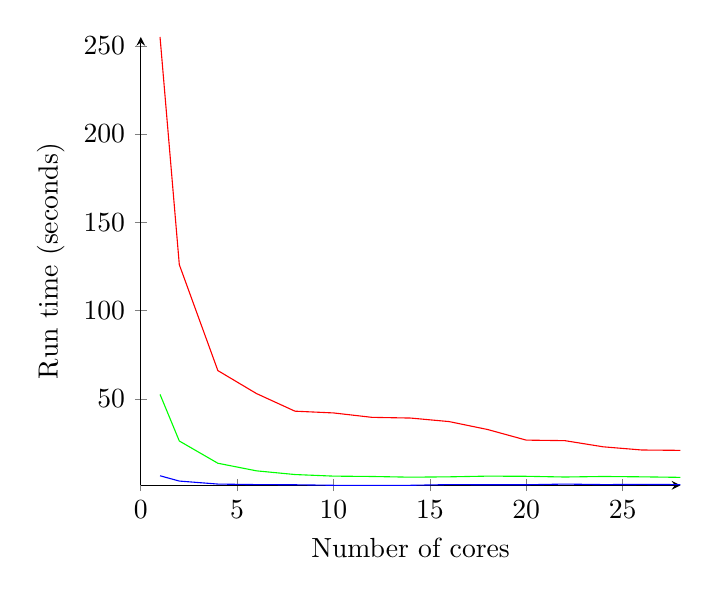
\begin{tikzpicture}
\begin{axis}[
  axis lines = left,
  xlabel = Number of cores,
  ylabel = Run time (seconds),
  xmin = 0,
  ymin = 1,
]
% 128x128
\addplot[color=blue] table {
  1   6.4
  2   3.4
  4   1.7
  6   1.4
  8   1.3
  10  1.0
  12  0.9
  14  1.0
  16  1.4
  18  1.3
  20  1.3
  22  1.7
  24  1.4
  26  1.5
  28  1.4
};

% 256x256 
\addplot[color=green] table {
  1   52.5
  2   26.1
  4   13.5
  6   9.2
  8   7.1
  10  6.2
  12  6.0
  14  5.6
  16  5.8
  18  6.2
  20  6.1
  22  5.7
  24  6.0
  26  5.8
  28  5.5
};

% 1028x1028
\addplot[color=red] table {
  1   255
  2   126
  4   66
  6   53
  8   43 
  10  42
  12  39.5
  14  39.1
  16  37.1
  18  32.6
  20  26.6
  22  26.3
  24  22.8
  26  21.0
  28  20.8
};
\end{axis}
\end{tikzpicture}
\captionof{figure}{Parallel scaling results for 1-28 cores}
\label{fig:parallelresults}

\begin{center}
  \begin{tabular}{ |p{1.5cm}||p{1.5cm}|p{1.5cm}|p{1.5cm}| }
 \hline
 \multicolumn{4}{|c|}{Results} \\
 \hline
 Number of cores & 128x128 & 256x256 & 1024x1024 \\
 \hline
 1  & 6.4 &  52.5  &  255.4   \\
 2  & 3.4 &  26.1  &  126.2   \\
 4  & 1.7 &  13.5  &  66.1    \\ 
 6  & 1.4 &  9.2   &  53.3    \\ 
 8  & 1.3 &  7.1   &  43.4    \\ 
 10 & 1.0 &  6.2   &  42.4    \\
 12 & 0.9 &  6.0   &  39.7    \\
 14 & 1.0 &  5.6   &  39.1    \\ 
 16 & 1.4 &  5.8   &  37.1    \\ 
 18 & 1.3 &  6.2   &  32.6    \\
 20 & 1.3 &  6.1   &  26.6    \\
 22 & 1.7 &  5.7   &  26.3    \\ 
 24 & 1.4 &  6.0   &  22.8    \\ 
 26 & 1.5 &  5.8   &  21.0    \\ 
 28 & 1.4 &  5.5   &  20.8    \\
 \hline
\end{tabular}
\captionof{table}{Parallel scaling results for 1-28 cores}
\label{tab:parallelresults}
\end{center}

\end{multicols}
\end{document}

